\section{Results}
\label{sec:results}

\subsection{Calibration (RQ1: H1a, H1b)}

Table~\ref{tab:calibration} shows that every probe except S1 kept its false-positive rate (FPR) close to $\alpha$ under exact permutation tests (0.033--0.058 over 240 null datasets; M3 0.100 over only 30, with an interval reaching 0.02). S1 never rejected. This is a resolution effect rather than good behaviour: with $m=25$ features and $B=100$ permutations, the smallest per-feature $p$-value ($1/101$) cannot clear the first Simes threshold $\alpha/m=0.002$. Per-feature permutation tests therefore need $B\ge m/\alpha$, here 500. Under the Monte Carlo null, all eleven probes had hold-out FPRs between 0.027 and 0.068, with every interval containing 0.05, and on a random 5\% sample of datasets the Monte Carlo and dataset-specific permutation $p$-values led to the same decision in 97.1\% of 210 comparisons (Spearman $\rho=0.989$). H1a is supported.

\begin{table}[!t]
\centering
\caption{False-positive rates at $\alpha=0.05$ on null data (number of null datasets in brackets).}
\label{tab:calibration}
\footnotesize
\begin{adjustbox}{max width=\linewidth}
\begin{tabular}{lcc}
\hline
Probe & Permutation FPR [95\% CI] & Monte Carlo FPR [95\% CI] \\ \hline
S1 MI & 0.000 [0.000, 0.015] (240) & 0.045 [0.022, 0.082] (220) \\
S2 ANOVA/$\chi^2$ & 0.046 [0.023, 0.081] (240) & 0.055 [0.028, 0.093] (220) \\
S3 dCor & 0.054 [0.029, 0.091] (240) & 0.050 [0.025, 0.088] (220) \\
S4 HSIC & 0.054 [0.029, 0.091] (240) & 0.055 [0.028, 0.093] (220) \\
G1 F1 & 0.037 [0.017, 0.070] (240) & 0.045 [0.022, 0.082] (220) \\
G2 N1 & 0.054 [0.029, 0.091] (240) & 0.064 [0.035, 0.104] (220) \\
G3 N3 & 0.058 [0.032, 0.096] (240) & 0.068 [0.039, 0.110] (220) \\
M1 Tree & 0.033 [0.014, 0.065] (240) & 0.050 [0.025, 0.088] (220) \\
M2 LogReg & 0.058 [0.032, 0.096] (240) & 0.055 [0.028, 0.093] (220) \\
M3 Forest & 0.100 [0.021, 0.265] (30) & 0.027 [0.010, 0.058] (220) \\
M4 HGB & 0.033 [0.001, 0.172] (30) & 0.032 [0.013, 0.064] (220) \\
\hline
\end{tabular}
\end{adjustbox}
\par\vspace{2pt}\parbox{0.95\linewidth}{\scriptsize Permutation: Experiment A1, dataset-specific label permutations. Monte Carlo: hold-out null datasets of Experiment B tested against the simulated null.}
\end{table}


Combining per-feature tests without correction was badly miscalibrated (Table~\ref{tab:multiple}): the FPR was 0.36--0.41 with 10 features, 0.90--0.95 with 50 and 1.00 with 200, closely tracking $1-0.95^p$. Simes/Benjamini--Hochberg aggregation brought it to 0.017--0.073, except for S1 at $n=200$ with 200 features (0.090, i.e.\ 27 of 300). H1b is supported.

\begin{table}[!t]
\centering
\caption{Experiment A2: false-positive rate of per-feature tests with and without multiple-testing correction (300 null datasets per row).}
\label{tab:multiple}
\footnotesize
\begin{adjustbox}{max width=\linewidth}
\begin{tabular}{lccccc}
\hline
Probe & $n$ & $p$ & Uncorrected & Simes/BH & $1-0.95^p$ \\ \hline
S1 MI & 200 & 10 & 0.413 & 0.033 & 0.401 \\
S1 MI & 200 & 50 & 0.903 & 0.047 & 0.923 \\
S1 MI & 200 & 200 & 1.000 & 0.090 & 1.000 \\
S1 MI & 1000 & 10 & 0.357 & 0.017 & 0.401 \\
S1 MI & 1000 & 50 & 0.947 & 0.030 & 0.923 \\
S1 MI & 1000 & 200 & 1.000 & 0.027 & 1.000 \\
S2 ANOVA/$\chi^2$ & 200 & 10 & 0.410 & 0.033 & 0.401 \\
S2 ANOVA/$\chi^2$ & 200 & 50 & 0.943 & 0.037 & 0.923 \\
S2 ANOVA/$\chi^2$ & 200 & 200 & 1.000 & 0.063 & 1.000 \\
S2 ANOVA/$\chi^2$ & 1000 & 10 & 0.403 & 0.060 & 0.401 \\
S2 ANOVA/$\chi^2$ & 1000 & 50 & 0.903 & 0.073 & 0.923 \\
S2 ANOVA/$\chi^2$ & 1000 & 200 & 1.000 & 0.050 & 1.000 \\
\hline
\end{tabular}
\end{adjustbox}
\end{table}


\subsection{Power and Signal Type (RQ1, RQ2: H1c, H2a)}

Fig.~\ref{fig:power} and Table~\ref{tab:power} show the central result: \emph{which probe is most powerful depends on the type of signal}. For linear signal, distance correlation and HSIC were strongest (mean power 0.78), closely followed by S2, F1 and logistic regression (0.74); their minimum detectable effect at $n=1000$ was a Bayes AUC of 0.59--0.64 (Table~\ref{tab:mde}). For nonlinear signal, whose classes differ in spread but not in mean, S2, F1 and logistic regression were blind (0.03), whereas the random forest (0.62), gradient boosting (0.58) and the shallow tree (0.52) detected it. For interaction-only signal, all per-feature probes stayed at the null level (maximum power: S1 0.12, S2 0.08, F1 0.08), supporting H2a. Only gradient boosting (0.49), the forest (0.36) and the neighbourhood measures N1/N3 (0.32) detected interaction signal, and only at $n\ge1000$; gradient boosting reached 80\% power at a Bayes AUC of 0.70 for $n=1000$ and 0.59 for $n=5000$.

\begin{figure*}[!t]
\centering
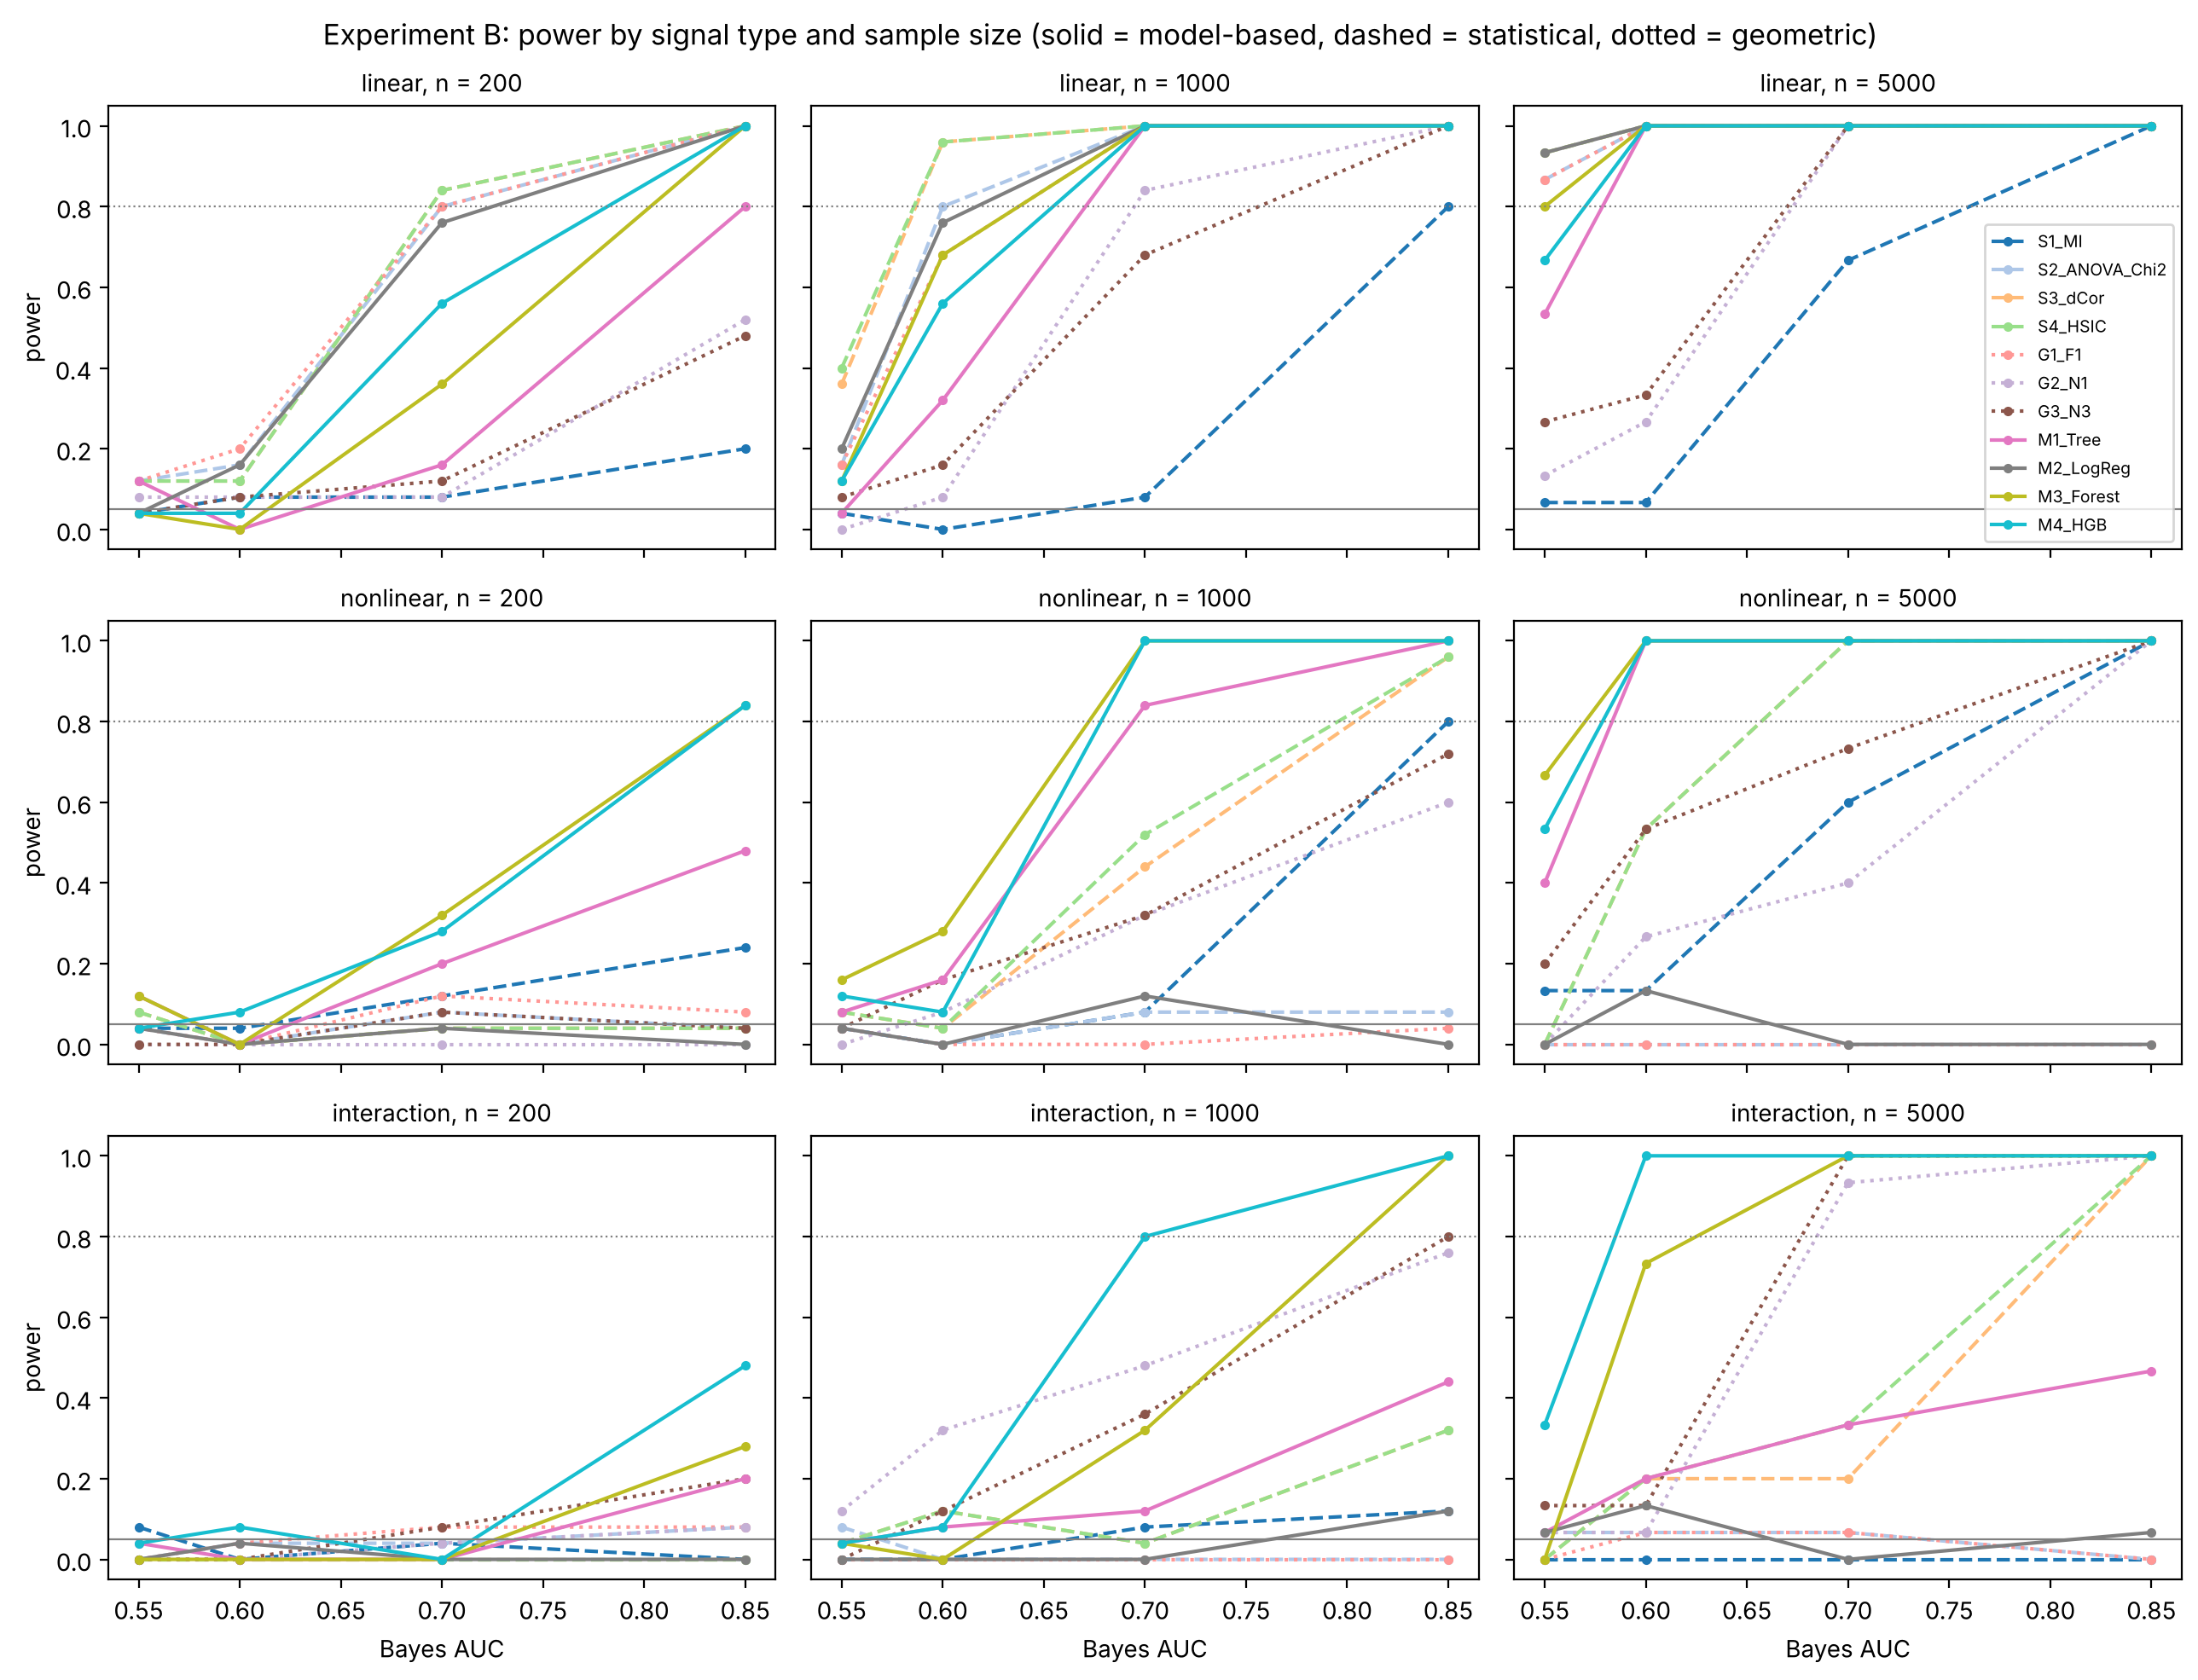
\includegraphics[width=0.92\textwidth]{../figures/expB_power_curves.png}
\caption{Experiment B: power against Bayes AUC by signal type (rows) and sample size (columns). Solid lines: model-based probes; dashed: statistical; dotted: geometric. Grey lines mark $\alpha=0.05$ and 80\% power.}
\label{fig:power}
\end{figure*}

\begin{table*}[!t]
\centering
\caption{Experiment B: mean power at $\alpha=0.05$, averaged over the four signal strengths (Bayes AUC 0.55--0.85).}
\label{tab:power}
\footnotesize
\begin{adjustbox}{max width=\linewidth}
\begin{tabular}{lccccccc}
\hline
Probe & All & Interaction & Linear & Nonlinear & $n$=200 & $n$=1000 & $n$=5000 \\ \hline
S1 MI & 0.19 & 0.03 & 0.26 & 0.27 & 0.08 & 0.17 & 0.31 \\
S2 ANOVA/$\chi^2$ & 0.27 & 0.04 & 0.74 & 0.03 & 0.20 & 0.27 & 0.34 \\
S3 dCor & 0.43 & 0.16 & 0.78 & 0.35 & 0.19 & 0.45 & 0.66 \\
S4 HSIC & 0.44 & 0.17 & 0.78 & 0.36 & 0.19 & 0.46 & 0.67 \\
G1 F1 & 0.26 & 0.03 & 0.74 & 0.03 & 0.21 & 0.24 & 0.33 \\
G2 N1 & 0.32 & 0.32 & 0.42 & 0.22 & 0.07 & 0.38 & 0.51 \\
G3 N3 & 0.36 & 0.32 & 0.44 & 0.32 & 0.09 & 0.37 & 0.61 \\
M1 Tree & 0.42 & 0.17 & 0.58 & 0.52 & 0.18 & 0.43 & 0.67 \\
M2 LogReg & 0.27 & 0.04 & 0.74 & 0.03 & 0.17 & 0.27 & 0.36 \\
M3 Forest & 0.55 & 0.36 & 0.67 & 0.62 & 0.25 & 0.55 & 0.85 \\
M4 HGB & 0.58 & 0.49 & 0.67 & 0.58 & 0.29 & 0.57 & 0.88 \\
\hline
\end{tabular}
\end{adjustbox}
\end{table*}


Across the 36 settings the probes differed strongly (Friedman $\chi^2=65.3$, $p=3.5\times10^{-10}$; Table~\ref{tab:ranks}); following~\cite{benavoli2016}, each probe was then compared with the best one by a Wilcoxon signed-rank test with Holm correction. Gradient boosting had the best mean rank (3.92). The random forest (Holm $p=0.41$), HSIC and distance correlation (both $p=0.091$) were not significantly worse; all other probes were. At $n=200$ every probe had low power (at most 0.29), with gradient boosting highest and F1 the best model-free probe (0.21). H1c is therefore supported in the narrow sense that a model-based probe was most powerful, but no probe is reliable at $n=200$ unless the signal is strong and linear.

\begin{table}[!t]
\centering
\caption{Ranking of probes over the 36 settings of Experiment B (Friedman $\chi^2=65.3$, $p=3.5e-10$). Gap and $p$-value refer to a Wilcoxon signed-rank comparison with the best-ranked probe, Holm-corrected.}
\label{tab:ranks}
\footnotesize
\begin{adjustbox}{max width=\linewidth}
\begin{tabular}{lccc}
\hline
Probe & Mean rank & Power gap to best & Holm $p$ \\ \hline
M4 HGB & 3.92 & -- & -- \\
M3 Forest & 4.54 & 0.029 & 0.406 \\
M1 Tree & 5.10 & 0.155 & 0.002 \\
S4 HSIC & 5.22 & 0.141 & 0.091 \\
S3 dCor & 5.32 & 0.149 & 0.091 \\
G3 N3 & 6.25 & 0.220 & 2.6e-04 \\
S2 ANOVA/$\chi^2$ & 6.61 & 0.309 & 0.009 \\
G1 F1 & 6.85 & 0.315 & 0.008 \\
G2 N1 & 6.97 & 0.256 & 2.8e-04 \\
M2 LogReg & 7.15 & 0.310 & 0.004 \\
S1 MI & 8.07 & 0.393 & 1.4e-05 \\
\hline
\end{tabular}
\end{adjustbox}
\end{table}


\begin{table*}[!t]
\centering
\caption{Minimum detectable effect: smallest Bayes AUC at which a probe reaches 80\% power (linear interpolation; ``$>0.85$'' = never within the tested range).}
\label{tab:mde}
\footnotesize
\begin{adjustbox}{max width=\linewidth}
\begin{tabular}{lccccccccc}
\hline
Probe & inter. 200 & inter. 1000 & inter. 5000 & lin. 200 & lin. 1000 & lin. 5000 & nonli. 200 & nonli. 1000 & nonli. 5000 \\ \hline
S1 MI & $>$0.85 & $>$0.85 & $>$0.85 & $>$0.85 & 0.850 & 0.760 & $>$0.85 & 0.850 & 0.775 \\
S2 ANOVA/$\chi^2$ & $>$0.85 & $>$0.85 & $>$0.85 & 0.700 & 0.600 & $\le$0.55 & $>$0.85 & $>$0.85 & $>$0.85 \\
S3 dCor & $>$0.85 & $>$0.85 & 0.812 & 0.694 & 0.587 & $\le$0.55 & $>$0.85 & 0.804 & 0.657 \\
S4 HSIC & $>$0.85 & $>$0.85 & 0.805 & 0.694 & 0.586 & $\le$0.55 & $>$0.85 & 0.795 & 0.657 \\
G1 F1 & $>$0.85 & $>$0.85 & $>$0.85 & 0.700 & 0.637 & $\le$0.55 & $>$0.85 & $>$0.85 & $>$0.85 \\
G2 N1 & $>$0.85 & $>$0.85 & 0.685 & $>$0.85 & 0.695 & 0.673 & $>$0.85 & $>$0.85 & 0.800 \\
G3 N3 & $>$0.85 & 0.850 & 0.677 & $>$0.85 & 0.756 & 0.670 & $>$0.85 & $>$0.85 & 0.738 \\
M1 Tree & $>$0.85 & $>$0.85 & $>$0.85 & 0.850 & 0.671 & 0.579 & $>$0.85 & 0.694 & 0.583 \\
M2 LogReg & $>$0.85 & $>$0.85 & $>$0.85 & 0.725 & 0.617 & $\le$0.55 & $>$0.85 & $>$0.85 & $>$0.85 \\
M3 Forest & $>$0.85 & 0.806 & 0.625 & 0.803 & 0.637 & $\le$0.55 & 0.838 & 0.672 & 0.570 \\
M4 HGB & $>$0.85 & 0.700 & 0.585 & 0.782 & 0.655 & 0.570 & 0.839 & 0.678 & 0.579 \\
\hline
\end{tabular}
\end{adjustbox}
\end{table*}


\subsection{Robustness (RQ2: H2b, H2c)}

Irrelevant features hurt the distance-based probes most (Table~\ref{tab:robust}). With balanced classes, power at Bayes AUC 0.70 fell from 0.99 to 0.35 for distance correlation, from 1.00 to 0.35 for HSIC, from 0.99 to 0.13 for N1 and from 0.88 to 0.08 for N3 as irrelevant features went from 0 to 200, an average drop of 0.74. The model-based probes fell by 0.29 on average (forest 1.00 to 0.60, gradient boosting 1.00 to 0.65), supporting H2b and agreeing with the known dimension sensitivity of distance- and kernel-based tests~\cite{ramdas2015}. Under 10\% positives, permutation tests stayed calibrated (largest pooled FPR 0.058), and the forest remained the most powerful probe (0.93, 0.75 and 0.44 for 0, 20 and 200 irrelevant features). The geometric neighbourhood measures were the most affected by imbalance (N1: 0.23 with no irrelevant features). H2c is supported.

\begin{table}[!t]
\centering
\caption{Experiment C: power at Bayes AUC 0.70 and $n=1000$, averaged over the three signal types, by number of irrelevant features. Left block: balanced classes; right block: 10\% positives.}
\label{tab:robust}
\footnotesize
\begin{adjustbox}{max width=\linewidth}
\begin{tabular}{lcccccc}
\hline
Probe & 0 & 20 & 200 & 0  & 20  & 200  \\ \hline
S1 MI & 0.35 & 0.08 & 0.04 & 0.33 & 0.09 & 0.07 \\
S2 ANOVA/$\chi^2$ & 0.36 & 0.36 & 0.35 & 0.44 & 0.37 & 0.29 \\
S3 dCor & 0.99 & 0.49 & 0.35 & 0.77 & 0.47 & 0.37 \\
S4 HSIC & 1.00 & 0.52 & 0.35 & 0.79 & 0.49 & 0.24 \\
G1 F1 & 0.39 & 0.33 & 0.35 & 0.44 & 0.36 & 0.25 \\
G2 N1 & 0.99 & 0.55 & 0.13 & 0.23 & 0.08 & 0.07 \\
G3 N3 & 0.88 & 0.45 & 0.08 & 0.28 & 0.09 & 0.04 \\
M1 Tree & 0.84 & 0.65 & 0.48 & 0.41 & 0.53 & 0.41 \\
M2 LogReg & 0.40 & 0.37 & 0.35 & 0.39 & 0.35 & 0.23 \\
M3 Forest & 1.00 & 0.77 & 0.60 & 0.93 & 0.75 & 0.44 \\
M4 HGB & 1.00 & 0.93 & 0.65 & 0.76 & 0.59 & 0.25 \\
\hline
\end{tabular}
\end{adjustbox}
\end{table}


\subsection{Cost (RQ3: H3)}

On Adult subsamples (Table~\ref{tab:runtime}), one observed statistic cost 0.007--0.23~s for F1, N3, S1, S2 and the tree, about 2~s for distance correlation, HSIC and the forest, 9~s for N1 (dominated by the minimum spanning tree) and 7.5~s for gradient boosting, against 20.2~s for one 5-fold cross-validation of gradient boosting on all 48{,}842 rows. Because model-free probes reuse their label-independent preparation, their complete permutation test with $B=200$ took 0.2--28.5~s; a model-based test costs roughly $(B+1)$ times one cross-validation. At $n=5000$, S2, F1, the tree, the forest and gradient boosting were Pareto-optimal in power versus cost. A model-free probe is thus on the front, but power for $n\ge10{,}000$ was not simulated, so H3 is only partly supported.

\begin{table*}[!t]
\centering
\caption{Wall-clock seconds for one observed statistic on Adult subsamples (2 CPU cores). Quadratic-cost probes use at most 5{,}000 rows and model-based probes at most 10{,}000.}
\label{tab:runtime}
\footnotesize
\begin{adjustbox}{max width=\linewidth}
\begin{tabular}{lccccc}
\hline
Probe & $n$=1,000 & $n$=5,000 & $n$=10,000 & $n$=20,000 & $n$=48,842 \\ \hline
S1 MI & 0.050 & 0.139 & 0.128 & 0.131 & 0.132 \\
S2 ANOVA/$\chi^2$ & 0.065 & 0.074 & 0.090 & 0.106 & 0.157 \\
S3 dCor & 0.071 & 1.839 & 1.770 & 2.106 & 1.956 \\
S4 HSIC & 0.085 & 1.736 & 1.927 & 2.025 & 1.800 \\
G1 F1 & 0.002 & 0.021 & 0.014 & 0.016 & 0.007 \\
G2 N1 & 0.248 & 9.304 & 9.418 & 10.198 & 8.996 \\
G3 N3 & 0.025 & 0.224 & 0.248 & 0.230 & 0.232 \\
M1 Tree & 0.025 & 0.086 & 0.158 & 0.158 & 0.174 \\
M2 LogReg & 0.102 & 0.382 & 0.632 & 0.642 & 0.629 \\
M3 Forest & 0.513 & 1.042 & 2.289 & 2.160 & 2.063 \\
M4 HGB & 2.626 & 4.929 & 7.064 & 6.823 & 7.492 \\
Ref.: HGB 5-fold CV & 2.472 & 5.033 & 7.219 & 8.573 & 20.196 \\
\hline
\end{tabular}
\end{adjustbox}
\end{table*}


\subsection{Real Distributions (RQ4: H4a, H4b)}

On the label-shuffled real datasets (Fig.~\ref{fig:semi}), every probe detected signal when at most half of the labels were shuffled. At $q=0.9$, distance correlation and HSIC still detected it in 62\% of replicates, S2 and F1 in about 40\%, and gradient boosting in 12\%. The signal in these four datasets is largely monotone in single features, which favours the dependence tests. At $q=1$ (exact null) the detection rate was 0--0.125 per probe (gradient boosting 5 of 40). All probe statistics tracked the retained signal fraction closely (mean Spearman $\rho$: statistical 0.960, model-based 0.953, geometric 0.940). The difference H4a predicted exists but is negligible, so H4a is only nominally supported.

\begin{figure*}[!t]
\centering
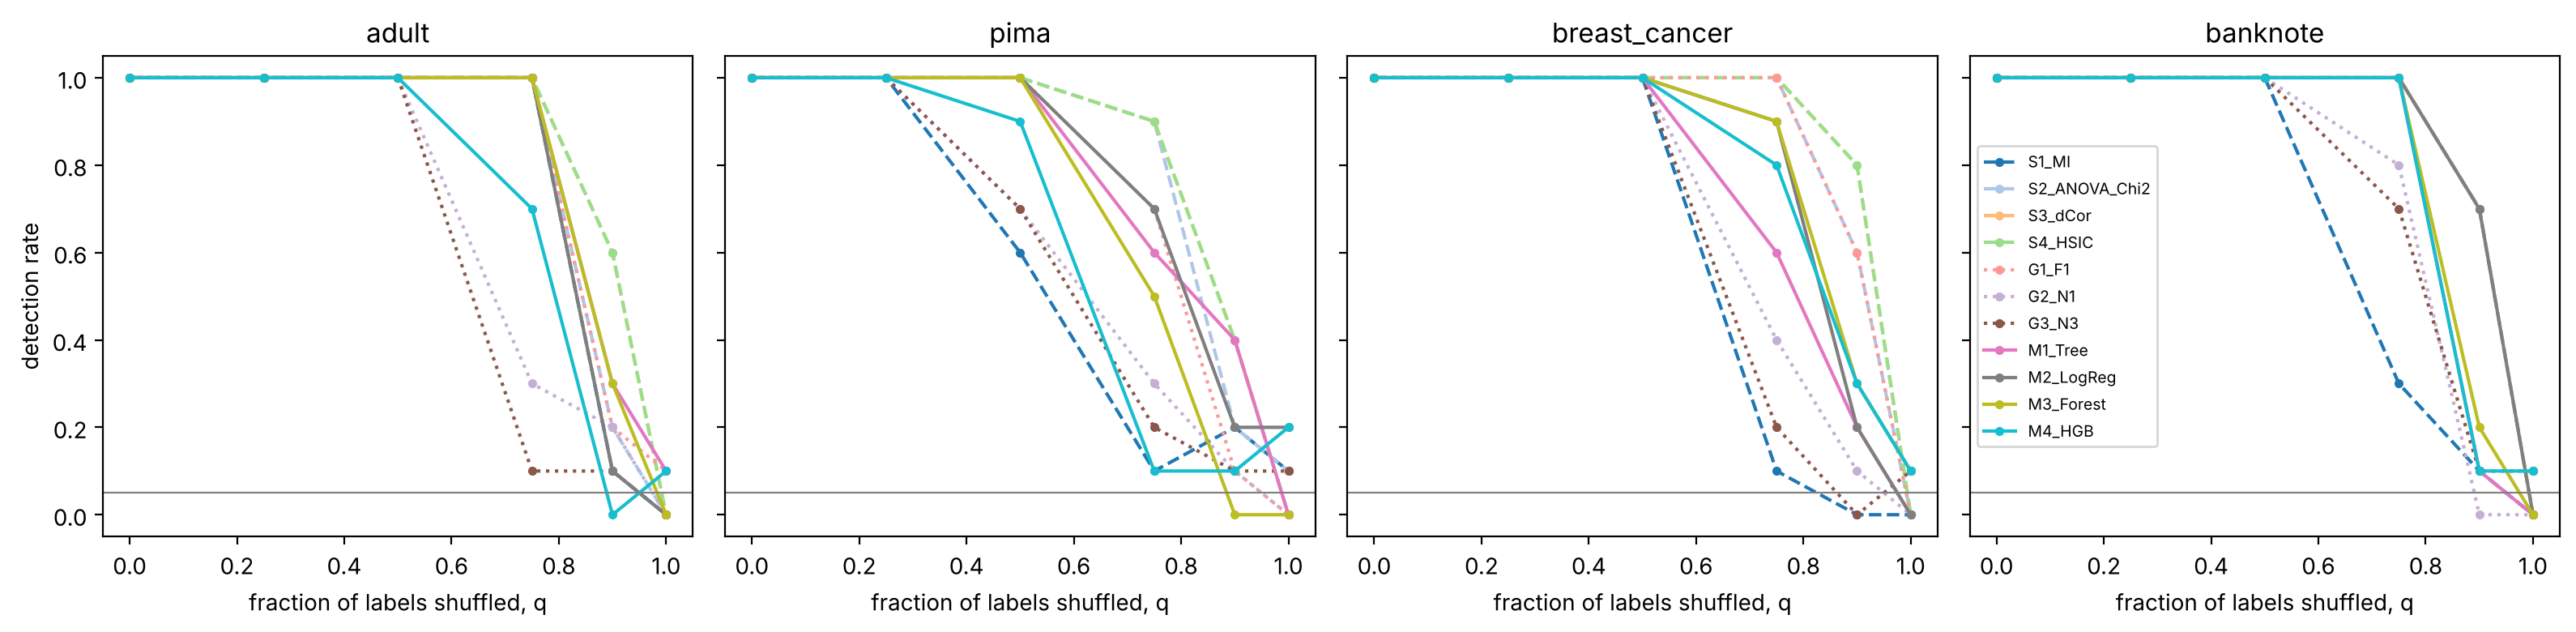
\includegraphics[width=0.95\textwidth]{../figures/semisynthetic_detection.png}
\caption{Semi-synthetic experiment: detection rate against the fraction $q$ of shuffled labels for each base dataset (10 replicates per point). At $q=1$ the labels are fully permuted, so the detection rate is the false-positive rate.}
\label{fig:semi}
\end{figure*}

Selected on Experiment~B alone, the two-stage protocol used HSIC (stage~1) and gradient boosting (stage~2). In Experiment~B its power was 0.519, slightly below gradient boosting alone (0.532), with a hold-out FPR of 0.027. On the semi-synthetic validation data its power was 0.890, well above gradient boosting (0.750) but below HSIC alone (0.920), with no false positives in 40 null replicates. The protocol therefore offers robustness to signal type rather than the highest power in any single scenario, and H4b is partly supported.

\subsection{Case Studies}

Table~\ref{tab:cases} reports every probe on the real datasets. On \textbf{Adult}, all probes rejected $H_0$ at their smallest attainable $p$-value, and the AUC gain over the dummy model on the full data was 0.428 for gradient boosting (95\% interval 0.428--0.429; AUC 0.928) and 0.405 for logistic regression. Learning curves showed logistic regression saturating at about 0.905 from 1{,}000 rows, while gradient boosting kept improving to 0.928, so additional data mainly benefits flexible models.

\begin{table*}[!t]
\centering
\caption{Case studies: permutation $p$-values of every probe (Adult: $B=200$, 40 for M3/M4; NSW: $B=1000$, 200; incentive experiment: $B=500$, 200).}
\label{tab:cases}
\footnotesize
\begin{adjustbox}{max width=\linewidth}
\begin{tabular}{lcccc}
\hline
Probe & Adult & NSW (randomised) & Thornton (randomised) & Thornton incl. village \\ \hline
S1 MI & 0.005 & 0.024 & 0.006 & 0.004 \\
S2 ANOVA/$\chi^2$ & $<$0.001 & 0.017 & 0.106 & $<$0.001 \\
S3 dCor & 0.005 & 0.019 & 0.032 & 0.002 \\
S4 HSIC & 0.005 & 0.036 & 0.026 & 0.002 \\
G1 F1 & 0.005 & 0.011 & 0.106 & 0.002 \\
G2 N1 & 0.005 & 0.901 & 0.162 & 0.002 \\
G3 N3 & 0.005 & 0.515 & 0.495 & 0.002 \\
M1 Tree & 0.005 & 0.027 & 0.012 & 0.010 \\
M2 LogReg & 0.005 & 0.033 & 0.038 & 0.002 \\
M3 Forest & 0.024 & 0.010 & 0.010 & 0.005 \\
M4 HGB & 0.024 & 0.368 & 0.005 & 0.005 \\
\hline
\end{tabular}
\end{adjustbox}
\end{table*}


The two \textbf{randomised experiments} were the most instructive cases. On \textbf{NSW}, eight of the eleven probes gave $p<0.05$, although the protocol's two stages did not reach $\alpha/2$ (HSIC $p=0.036$, gradient boosting $p=0.368$), so the protocol returned ``no signal detected''. The per-feature test traced the dependence to the no-degree indicator ($p=0.0021$, the only feature rejected by Benjamini--Hochberg; standardised mean difference $-0.30$). This is a chance imbalance in the subsample rather than a design feature, and the cross-validated AUC gains were small (logistic regression 0.056).

On the \textbf{incentive experiment} with individual covariates only, gradient boosting ($p=0.005$, AUC gain 0.058) and the forest ($p=0.010$) detected dependence, and the protocol returned ``signal detected''. With village included, every probe rejected $H_0$ ($p\le0.01$; logistic-regression gain 0.177). Two diagnostics explain part of this. Distance alone identified a person's village with 44\% accuracy, against 4.4\% for the most common village. Under a design-aware test that permutes labels only within villages, distance correlation was no longer significant ($p=0.35$, against 0.025 under ordinary permutation). The tree ensembles, however, stayed significant (forest $p=0.035$, gradient boosting $p=0.015$), which points to further design structure that the public data do not document. In short, ``null by design'' is a claim about the design, and the probes found that it did not hold exactly in either randomised dataset.

\subsection{Ojala--Garriga Replication}

Table~\ref{tab:ojala} and Fig.~\ref{fig:ojala} summarise both tests. Test~1 was significant ($p=0.005$, the minimum) for all four classifiers on Adult, Pima, Banknote, Breast Cancer and the synthetic linear data, and non-significant for every classifier on Adult with permuted labels ($p\ge0.60$), NSW ($p\ge0.06$) and the incentive experiment with individual covariates ($p\ge0.10$). The interaction-only data separated the classifiers: the unpruned tree ($p=0.25$) and naive Bayes ($p=0.82$) missed the signal, whereas 1-NN ($p=0.035$) and the SVM ($p=0.005$) detected it. For exactly those two, Test~2 was also significant ($p=0.005$), correctly identifying that their signal lies in a dependency between features. Test~2 was also significant for the tree, 1-NN and SVM on Banknote, but not on Adult, Pima or Breast Cancer, where within-class permutation did not increase the error ($p\ge0.84$), consistent with signal carried by individual features.

\begin{table*}[!t]
\centering
\caption{Ojala--Garriga replication: accuracy / Test~1 $p$ / Test~2 $p$ per classifier (10-fold CV, $k=200$ permutations; smallest attainable $p$ = 0.005).}
\label{tab:ojala}
\footnotesize
\begin{adjustbox}{max width=\linewidth}
\begin{tabular}{lcccc}
\hline
Dataset & DT & NB & 1NN & SVM \\ \hline
Adult (n=2000) & 0.81 / 0.005 / 1.000 & 0.33 / 0.005 / 1.000 & 0.79 / 0.005 / 1.000 & 0.85 / 0.005 / 1.000 \\
Pima & 0.70 / 0.005 / 0.920 & 0.76 / 0.005 / 1.000 & 0.71 / 0.005 / 0.846 & 0.76 / 0.005 / 1.000 \\
Banknote & 0.99 / 0.005 / 0.005 & 0.84 / 0.005 / 1.000 & 1.00 / 0.005 / 0.005 & 1.00 / 0.005 / 0.005 \\
Breast cancer & 0.92 / 0.005 / 1.000 & 0.94 / 0.005 / 1.000 & 0.95 / 0.005 / 1.000 & 0.98 / 0.005 / 1.000 \\
Synthetic linear & 0.61 / 0.005 / 0.075 & 0.70 / 0.005 / 0.398 & 0.60 / 0.005 / 0.219 & 0.68 / 0.005 / 0.458 \\
Synthetic interaction & 0.51 / 0.249 / 0.383 & 0.48 / 0.821 / 0.965 & 0.54 / 0.035 / 0.005 & 0.64 / 0.005 / 0.005 \\
NSW (randomised) & 0.51 / 0.667 / 0.876 & 0.58 / 0.070 / 0.318 & 0.51 / 0.597 / 0.776 & 0.60 / 0.060 / 0.468 \\
Thornton (randomised) & 0.65 / 0.100 / 0.806 & 0.77 / 0.572 / 1.000 & 0.65 / 0.100 / 0.308 & 0.77 / 0.866 / 0.915 \\
Adult, permuted labels & 0.62 / 0.791 / 0.746 & 0.25 / 0.851 / 0.239 & 0.63 / 0.607 / 0.627 & 0.76 / 0.851 / 0.995 \\
Thornton incl. village & 0.68 / 0.005 / 0.597 & 0.34 / 0.015 / 0.915 & 0.68 / 0.005 / 0.453 & 0.76 / 0.905 / 0.592 \\
\hline
\end{tabular}
\end{adjustbox}
\end{table*}


\begin{figure*}[!t]
\centering
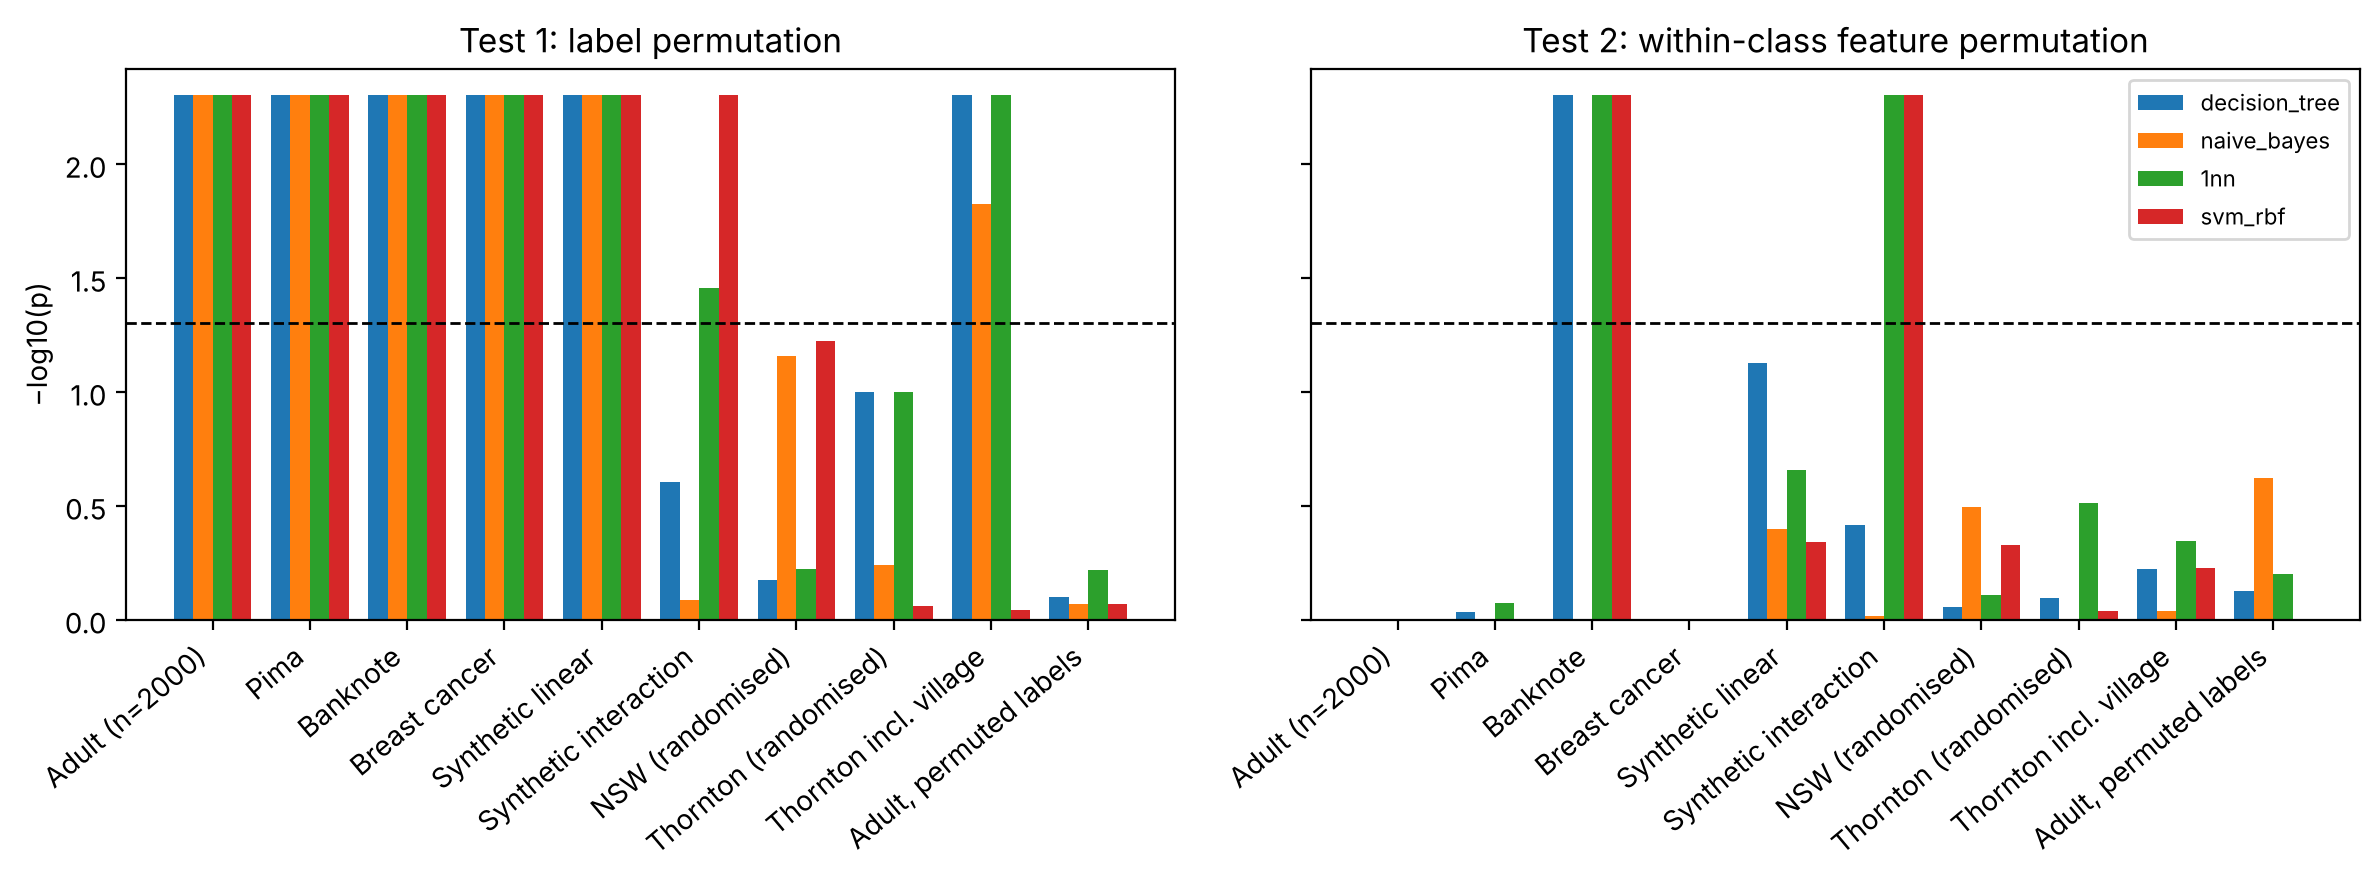
\includegraphics[width=0.92\textwidth]{../figures/ojala_garriga.png}
\caption{Ojala--Garriga Tests 1 and 2: $-\log_{10}p$ per classifier and dataset ($k=200$ permutations; ceiling 2.3). Dashed line: $p=0.05$.}
\label{fig:ojala}
\end{figure*}

Accuracy-based Test~1 and the AUC-based model probes disagreed on the incentive experiment (77\% positives): no classifier's accuracy beat its permutation distribution, whereas gradient boosting's AUC did ($p=0.005$). Under imbalance, accuracy is dominated by the majority class, so AUC is the more sensitive statistic.

\subsection{Leakage}

The sanity check (Table~\ref{tab:sanity}) flagged the identifier column, the crude leak (single-feature AUC 0.995) and the incentive amount in the incentive experiment (AUC 1.000). It passed the subtle leak (a copy of $y$ with 10\% flipped values, AUC 0.90), on which every probe rejected $H_0$ ($p\le0.026$), and it passed NSW with the post-treatment earnings \texttt{re78}. A clean sanity check is therefore no guarantee: post-outcome features must be excluded by reasoning about when each variable was measured.

\begin{table}[!t]
\centering
\caption{Experiment D: sanity check verdicts.}
\label{tab:sanity}
\footnotesize
\begin{adjustbox}{max width=\linewidth}
\begin{tabular}{llcc}
\hline
Case & Sanity verdict & Best single feature & Its AUC \\ \hline
Null synthetic (control) & clean & x7 & 0.543 \\
Null + identifier column & leakage suspected & x7 & 0.543 \\
Null + crude leak (0.5\% flipped copy of y) & leakage suspected & leak & 0.995 \\
Null + subtle leak (10\% flipped copy of y) & clean & leak & 0.900 \\
NSW pre-treatment only & clean & nodegree & 0.563 \\
NSW + re78 (post-treatment) & clean & re78 & 0.570 \\
Thornton pre-treatment only & clean & age & 0.523 \\
Thornton + village & clean & villnum & 0.659 \\
Thornton + tinc (incentive amount) & leakage suspected & tinc & 1.000 \\
Adult & clean & relationship & 0.778 \\
Pima & clean & glucose & 0.788 \\
Banknote & clean & variance & 0.927 \\
Breast cancer & clean & worst\_perimeter & 0.975 \\
\hline
\end{tabular}
\end{adjustbox}
\end{table}


\FloatBarrier
\section{Discussion}
\label{sec:discussion}

Table~\ref{tab:verdicts} summarises the hypothesis verdicts. Four findings matter most for practice.

\textbf{No single family is sufficient.} Linear dependence tests (S2, F1, logistic regression) are efficient for additive signal but blind to signal that changes spread or lives in interactions, and the latter is exactly where flexible learners are needed. Distance correlation and HSIC are the best model-free compromise, but they degrade quickly with irrelevant features. Gradient boosting had the best overall rank, yet on the real, largely monotone datasets it was the least powerful model-based probe. Pairing a multivariate dependence test with a flexible learner is therefore a reasonable default, and Ojala--Garriga's Test~2 adds a cheap diagnostic of \emph{where} the signal lives.

\textbf{Calibration is easy; aggregation and resolution are not.} Permutation wrapping made every probe's false-positive rate exact, including the descriptive complexity measures, which have no null distribution of their own (gap G2). The two practical traps are combining per-feature tests without correction, which raised the FPR to 0.90 with 50 features, and using too few permutations for a per-feature test, which made S1 unable to reject at all.

\textbf{Small samples are the hard case.} At $n=200$ no probe exceeded 0.29 mean power, and most signals with Bayes AUC below 0.7 went undetected. A ``no signal detected'' verdict at that size says little unless it carries the MDE: for example, gradient boosting at $n=1000$ detects interaction signal only above a Bayes AUC of about 0.70.

\textbf{``No signal by design'' must be verified.} Both randomised experiments carried detectable dependence: a chance covariate imbalance in NSW, and assignment probabilities that varied by village in the incentive experiment. The probes behaved correctly; the assumption was wrong. For practitioners this cuts both ways: a probe that rejects $H_0$ shows that the target depends on the features in \emph{this sample}, which is not the same as stable, useful signal. Effect sizes (NSW: AUC gain about 0.05) and design-aware nulls such as within-stratum permutation should accompany the verdict.

\begin{table}[!t]
\centering
\caption{Verdicts on the pre-registered hypotheses.}
\label{tab:verdicts}
\footnotesize
\begin{adjustbox}{max width=\linewidth}
\begin{tabular}{lp{5.3cm}l}
\hline
Hypothesis & Statement & Verdict \\ \hline
H1a & Permutation-wrapped probes are calibrated & supported \\
H1b & Uncorrected per-feature aggregation inflates FPR; Simes/BH restores it & supported \\
H1c & Model-based probes most powerful at small n & supported \\
H2a & Per-feature probes blind to interaction-only signal & supported \\
H2b & Distance-based probes lose power faster with irrelevant features & supported \\
H2c & AUC-based probes stay calibrated and useful under 10:90 imbalance & supported \\
H3 & A model-free probe is Pareto-optimal at large n & partly supported \\
H4a & Model-based effect sizes track true strength better than geometric scores & nominal only (difference $<$ 0.02) \\
H4b & Two-stage protocol $\ge$ best single probe in power with FPR $\le$ $\alpha$ & partly supported \\
\hline
\end{tabular}
\end{adjustbox}
\end{table}


\textbf{Limitations.} Compute restrictions (two CPU cores, no GPU, GitHub-only network access) forced three deviations from the proposal: a random forest replaced TabPFN, scikit-learn's histogram gradient boosting replaced LightGBM, and power was simulated only up to $n=5000$ with 15--25 replicates per setting, which gives power estimates a standard error of up to 0.1. Synthetic features were Gaussian, so the categorical and mixed-type behaviour of the probes was tested only on the real datasets. Only binary targets and exchangeable rows were considered. Finally, the protocol's stages were selected on synthetic data whose signal types differ from those in the real datasets, which explains part of the gap between design and validation power.

\section{Conclusion}
\label{sec:conclusion}

Whether a tabular dataset holds learnable signal can be tested cheaply and with exact error control by wrapping statistical, geometric or model-based probes in a shared permutation layer. Across controlled, semi-synthetic and real data, the probes' power depended mainly on the type of signal: dependence tests excelled at linear signal, flexible learners at nonlinear and interaction signal, and neighbourhood complexity measures were sensitive to irrelevant features. A two-stage protocol (HSIC, then gradient boosting, Bonferroni-split) kept the false-positive rate below $\alpha$ and was robust across signal types, though not the most powerful choice in every scenario. The replication of Ojala and Garriga's tests showed that Test~2 reliably reveals interaction signal. Datasets that were null by design, finally, turned out not to be null in the sample, a reminder that the verdict ``signal detected'' always needs an effect size and a check of the design behind the data. Future work should add tabular foundation models, regression targets and power estimates for $n>5000$.
